\section{Production and Assembly}
\label{sec:fdsp-tpcelec-production}

In this section, we discuss the production and assembly plans,
including the plans for the spares required during the detector
construction and for operations, for
procurement, assembly, and quality control.

%%%%%%%%%%%%%%%%%%%%%%%%%%%%%%%%%%%

\subsection{Spares Plan}
\label{sec:fdsp-tpcelec-production-spares}

The \dword{apa} consortium plans on building 152 \dword{apa}s
for the first \dword{sp} detector. This means that at least
3,040 \dwords{femb} with the corresponding bundles of cold
cables will be required for the integration (3,040 power cables, 3,040 data cables,
and 1,216 bias voltage cables; half the cables will be long enough for 
integration on the top \dword{apa}s, while the other half will
be compatible with the bottom \dword{apa}s). To have spare \dwords{femb}, the \dword{tpc} electronics consortium plans to
build at least 3,200 \dwords{femb}, 5\% more than necessary. If more spares are needed during the
\dword{qc} process or during integration, additional 
\dwords{femb} can be produced quickly as long as any components that have 
long lead times are on hand. For these components, we plan to keep on hand a
larger number of spares. The \dwords{asic} require a long lead time; a plan for those spares is
discussed below. For other discrete components
(capacitors, resistors, connectors, voltage regulators, oscillators),
plans will be put in place once the final design of the \dword{femb}
is available and vendors contacted. %Please note that the
%size of the \dword{femb} production is such that the total number
%of some components exceeds the usual stock of some distributors.

For the \dwords{asic}, the number of spare chips is driven by the fact that fabrication
requires batches of 25 wafers at a time. Given the dimensions of the current prototype \dwords{asic}, the
expected number of chips per wafer is about 700 for \dword{larasic}, 930 for \dword{coldadc},
230 for \dword{coldata}, and 220 for \dword{cryo}. These numbers are based on the
assumption that \dword{coldadc} and \dword{coldata} are fabricated on the same wafer. To
estimate the number of usable chips for installation on the \dwords{femb}, we assume that
10\% of the chips will fail during the \dword{qc} process described later in this section,
and an additional 5\% of the chips will fail during dicing and packaging. With these
assumptions, one would need at least 43 \dword{larasic} wafers, 33 \dword{coldadc} and 
\dword{coldata} wafers, and 35 \dword{cryo} wafers for one \dword{sp} \dword{fd} module. Wafers
must be ordered in batches of 25 which implies that we will have a significant number of
spares, meaning that additional batches of wafers would be needed only if the overall
yield of \dword{larasic} falls below 75\% or if the overall yield of the other
\dwords{asic} falls below 60\%. The number of spare chips available can be reduced if wafers are purchased for two
\dword{sp} detectors at a time; however, the wafers are relatively inexpensive and the chosen
processes may not be available after a few years so generous spares of these custom devices
are likely advisable. 

In general, for other components, we plan to procure between 5 and
10\% additional components for spares for the construction of the first \dword{sp}
\dword{fd} module. We will need more spares for components that have
a larger risk of damage during integration and 
installation. For example, for cold cables, we
plan for 10\% additional spare cables for the bottom \dword{apa} because
they must be routed through the \dword{apa} frames, but
for the top \dword{apa}, we foresee needing only 5\% additional spare cables.
Assuming we will have unused spares from the first detector, we will reduce the number of
spares for the second \dword{sp} \dword{fd} module.

The components on top of the cryostat (power supplies, bias
voltage supplies, cables, \dwords{wiec} with their \dword{wib}
and \dword{ptc} boards) can be replaced while the
detector is in operation. For these components, additional spares may be required
during the \dunelifetime operation period of the \dword{dune} \dword{fd}.
The initial plan is to purchase 10\% additional components for spares for the first
\dword{sp} \dword{fd} module and use them for the second  \dword{sp} \dword{fd} as well
(i.e. effectively having 5\% additional components for spares). Once the design of
the \dwords{wib} is finalized, we will decide if 
extra spares should be purchased for \dwords{fpga} and optical
transmitters and receivers. These are commercial components 
that may no longer be available after a certain number of 
years of operation, which could prevent the \dword{tpc} electronics consortium from
fabricating additional spare \dwords{wib} if required. This
risk is discussed in Section~\ref{sec:fdsp-tpcelec-risks-operations}, one that
could be alleviated by placing commercial components
on mezzanine cards to minimize any necessary redesign of
boards if these components are no longer available.
We can also stock additional components
if market trends show that the components will  
become harder or impossible to find in the future.

%%%%%%%%%%%%%%%%%%%%%%%%%%%%%%%%%%%
\subsection{Procurement of Parts}
\label{sec:fdsp-tpcelec-production-procurement}

The construction of the detector components for \dword{dune} requires many large procurements that 
must be carefully planned to avoid delays. For the \dwords{asic}, the 
choice of vendor(s) is made at the time the technology used in designing 
the chips is chosen. For almost all other components, several vendors 
will bid on the same package. Depending on the requirements of the funding
agency and of the responsible institution, this may require a lengthy
selection process. The cold cables used to transmit data from the
\dwords{femb} to the \dwords{wib} represent a critical case. In this case
a technical qualification, including tests of the entire cold chain (from the \dword{femb}
to the receiver on the \dword{wib}) is required. Another problem is the 
large numbers of components required. In some cases, the number of components 
of a given type (resistors, capacitors) may far exceed the number of components
that the usual resellers keep in stock. This will 
require careful planning to avoid stopping the assembly chain for
the \dwords{femb}, for example, because 
one kind of component runs short. Figures~\ref{fig:sp-tpcelec-partsflow1}
and \ref{fig:sp-tpcelec-partsflow2} show the flow of the \dword{tpc}
electronics detector components through procurement, assembly,
\dword{qc} testing, and finally integration and installation at 
\dword{surf} using a color code to indicate the activities that
are performed by external vendors, those that take place at one of
the consortium institutions, and those that take place at \dword{surf}.

\begin{dunefigure}
[Parts flow for the detector components inside the cryostat]
{fig:sp-tpcelec-partsflow1}
{Parts flow for the TPC electronics detector components installed inside the cryostat.}
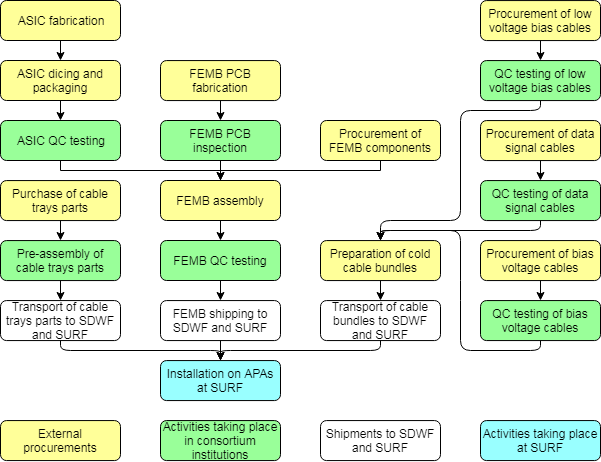
\includegraphics[width=0.8\linewidth]{sp-tpcelec-partsflow1.png}
\end{dunefigure}


%%%%%%%%%%%%%%%%%%%%%%%%%%%%%%%%%%%
\subsection{Assembly}
\label{sec:fdsp-tpcelec-production-assembly}

The \dword{tpc} electronics consortium plans to minimize
the amount of assembly work at any one of the participating
institutions. When assembly work is required, it will be performed
by external companies; examples are the installation of surface 
mount components, \dwords{asic}, \dwords{fpga} on the printed 
circuit boards for the \dwords{femb} and the \dwords {wib}, and
the assembly of the crossing tube cable supports. One of the few
exceptions is the assembly of the \dwords{wiec} that involves
mechanical and electrical connections at the backplane and crate supports.
Other activities that require 
work performed at one of the consortium institutions are the
assembly of the plugs attached to the cold cables, which are used to protect
the \dwords{femb} from \dword{esd} damage, and the preparation of
the bundles of low-voltage power, clock signal, trigger, data readout,
and bias voltage cables. During the engineering
phase and for components fabricated in small quantities, 
like boards used for testing other components, the plan is to
have one of the consortium's institutions assemble the components.
After assembly and testing, discussed below in Section~\ref{sec:fdsp-tpcelec-production-qc},
all detector components are shipped to the \dword{sdwf} and
later to \dword{surf}, where the final detector assembly
takes place as discussed in Chapter~\ref{ch:sp-install}.

%%%%%%%%%%%%%%%%%%%%%%%%%%%%%%%%%%%
\subsection{Quality Control}
\label{sec:fdsp-tpcelec-production-qc}

Once the \dword{apa}s are installed inside the cryostat, only
limited access to the detector components will be available to the \dword{tpc} electronics
consortium. After the \dword{tco} is closed, no access to detector
components will be available; therefore, they should be constructed to
last the entire lifetime of the experiment (\dunelifetime). This
puts very stringent requirements on the reliability of these
components, which has been already addressed in part through 
the \dword{qa} program discussed in Section~\ref{sec:fdsp-tpcelec-qa}. The
next step is to carefully apply stringent \dword{qc} procedures for  
detector parts to be installed in the detector.
All detector components installed inside the cryostat will
be tested and sorted before they are prepared for integration
with other detector components prior to installation. The full
details of the \dword{qc} plan have not been put in place
yet, and the specific selection criteria for the components will
be defined only after the current design and
prototyping phase is completed. For each detector component, a preliminary
version of the \dword{qc} program will be developed before the corresponding 
engineering design review. The program will then be used for
qualification of components fabricated during 
pre-production. It will be modified as needed before the production
readiness review that triggers the start of production of detector components
used for assembling the detector. In most cases the \dword{qc} program
will be informed by the experience gained with the tests of the corresponding
parts fabricated for \dword{pdsp}. Yields from the testing of \dword{larasic}
and of other discrete components mounted on the \dwords{femb} are discussed 
below. 

Some of the requirements for the \dword{qc} plans can
be laid out now based on the lessons learned
from constructing and commissioning the \dword{pdsp}
detector. Experience with \dword{pdsp} shows that a small fraction
(roughtly \num{4}\%) of the \dword{larasic} chips that pass the
qualification criteria at room temperature fail the tests
when immersed in \lntwo. Therefore, we plan to test all \dwords{asic} in \lntwo
before they are mounted on the \dwords{femb}; 
cryogenic testing of the \dwords{femb} is also planned. The goal of testing 
the \dwords{asic} in \lntwo is to minimize the need
to rework the \dwords{femb}. This is more important if 
the three \dwords{asic} solution is chosen for the
\dword{femb}. Since in this case there are 18 \dwords{asic} on the
\dword{femb}, an upper limit of 2\% on the fraction of
\dwords{femb} that require reworking translates into a requirement 
of less than 0.1\% of the \dwords{asic} failing during immersion in \lntwo.
If the \dword{cryo} solution is chosen for the \dwords{asic}
to be used on the \dwords{femb}, the 2\% requirement for the
number of \dwords{femb} to be reworked changes to a 
maximum failure rate of 1\%, given that there are only two
\dwords{asic} on the \dwords{femb}. Based on experiences at \dwords{pdsp},
discrete components like resistors and capacitors
need not undergo cryogenic testing before they are installed
on the \dwords{femb}. Capacitors and resistors are commonly
sold in reels of a few thousand components, which
should be typically sufficient for the fabrication of ten
\dwords{femb}. For these components, we are planning to
perform cryogenic tests on samples of a few components
from each reel prior to using the reel in the assembly of
\dwords{femb}. Some other components installed on
the \dwords{femb}, like voltage regulators and crystal oscillators, 
will have to be qualified like the \dwords{asic}
in \lntwo before being mounted on the \dwords{femb}. In the
case of the voltage regulators, it was found that the number
of failures were negligible and that cryogenic testing was
not necessary. One component used for \dword{pdsp}
that we are not planning to use for the \dword{dune} \dword{fd} \dwords{femb},
the memory card used to store the \dword{fpga} programming,
had instead a very high failure rate ($>50$\%).

\begin{dunefigure}
[Parts flow for the detector components on top of the cryostat]
{fig:sp-tpcelec-partsflow2}
{Parts flow for the TPC electronics detector components installed on top of the cryostat.}
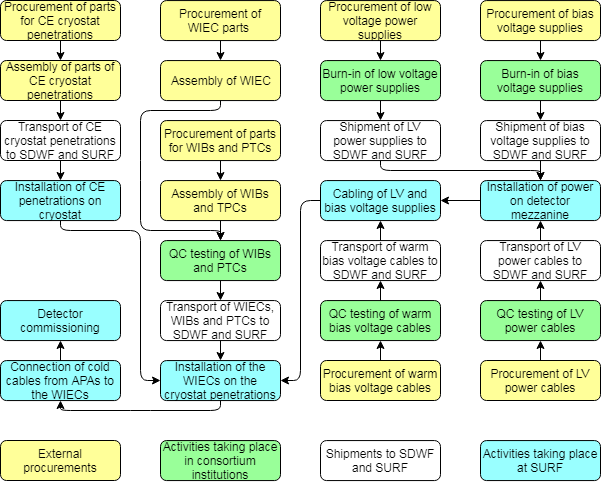
\includegraphics[width=0.8\linewidth]{sp-tpcelec-partsflow2.png}
\end{dunefigure}

\dword{asic} testing is performed with dedicated test boards that
allow tests of the functionality of the chips and are also used
to determine the initial calibration constants that are stored in
a database for later use. The dedicated test boards reproduce the
entire readout chain where the input to the \dword{fe} amplifier
or to the \dword{adc} is replaced by an appropriate signal generator,
and some parts of the backend may be replaced by a simple \dword{fpga}
that is directly connected to a computer. Tests of the \dwords{femb}
can be performed by connecting them directly to a standalone \dword{wib},
as discussed in Section~\ref{sec:fdsp-tpcelec-design-warm}. Given
the large number of \dwords{asic} and \dwords{femb} required for
one \dword{dune} \dword{fd} \dword{sp} detector, we plan to distribute the 
corresponding \dword{qc} activities among multiple institutions
belonging to the \dword{tpc} electronics consortium. Up to six
test sites are needed for the \dwords{asic} plus an additional
five sites for the \dwords{femb}, with each test 
equipped with a cryogenic system such as the \dword{cts}. All tests
will be performed following a common set of instructions.

The choice of distributing the testing activities among multiple
institutions has been made based in part on the experience gained
with \dword{pdsp}, where all associated testing activities were concentrated
at \dword{bnl}. While this approach had some advantages, like the direct availability
of the engineers that had designed the components, a strict conformance
to the testing rules, and a fast turn-around
time for repairs, it also required a very large commitment of
personnel from a single institution. Personnel from other institutions
interested in the \dword{tpc} electronics participated in the test
activities but could not commit for long periods of time. For
this reason, we are planning to distribute the \dword{qc} testing
activities for \dwords{asic} and \dwords{femb} among multiple
institutions belonging to the \dword{tpc} electronics consortium.
It should be noted that this approach is used in the \dword{lhc}
experiments for detector components like the silicon tracker 
modules where both the assembly and \dword{qc} activities take
place in parallel at multiple (of the order of ten) institutions.
To ensure that all sites produce similar
results, we will emphasize training experienced personnel
that will overview the testing activities at each site,
and we will have a reference set of \dwords{asic} and \dwords{femb}
that will be initially used to cross-calibrate the
test procedures among sites and then to check the
stability of the test equipment at each site. 
All testing activities for \dwords{asic} and \dwords{femb}
will be monitored by a member of the management of the \dword{tpc}
consortium who will also have the responsibility of training the
personnel at all sites and conducting site
inspections to ensure that all safety and testing rules
and procedures are applied uniformly. Test results will
be stored in a database, and criteria will be developed
for the acceptance of \dwords{asic} and \dwords{femb}. The acceptance rate
will be monitored, and in case of problems,
the failures will be analyzed and root cause analyses
will be performed. If necessary, the test program will be stopped
at all sites while issues are being investigated. In the case of \dword{cryo},
since each \dword{femb} will only have two chips, it may be possible to bypass
chip-level testing altogether. If the chip-level failure rate is low enough,
it may be sufficient to simply test assembled \dwords{femb} and reject or rework
those that fail the tests.

For the large numbers of
\dwords{asic} required for one \dword{dune} \dword{fd} \dword{sp} detector
(6,000 or 54,000 chips depending on the \dword{asic} solution
chosen), manual testing of the chips requires excessive 
amounts of resources and, based on the lessons learned from  
constructing  \dword{pdsp}, would lead to unacceptable rejection
factors. Ideally, the entire testing
process would be performed using a robotic system, where 
a robotic arm picks up the \dword{asic} from a tray, places
it on a test board, and holds it in place while the test
is performed, followed by sorting it into a second tray
based upon the test result. The requirement that the test
be performed in \lntwo prevents us from using this
scheme. Two of the biggest problems observed during the
construction of \dword{pdsp} were related to the \dword{qc}
of \dwords{asic} in \lntwo. The first one, related to
condensation on the test boards, has been addressed with
the development of the \dword{cts}, discussed in Section~\ref{sec:fdsp-tpcelec-qa-initial}.
The second one is related to placement of the chips into the
sockets on the test boards, and leads to test failures
and in some cases damage to the chips and/or the sockets.
To overcome problems with the manual placement of the chips into
the sockets, we plan to develop a robotic system
to perform this operation. Once the \dwords{asic} are 
placed on test boards, they will be moved manually into 
upgraded versions of the current \dword{cts} that can
house multiple test boards. At the end of the testing
procedure, the robotic system will then remove
the chips from the test boards and sort them according to
the test results. Based on the experience with the tests of
the \dword{pdsp} \dwords{asic}, as well as from other experiments,
we plan to have the sockets on the test boards cleaned on a regular 
basis and then replaced after a certain number of
testing cycles. 

Before assembly, the printed circuit boards for the
\dwords{femb} will be tested by the production vendor for electrical
continuity and shorts. The usual approach for particle physics
experiments is to perform a visual inspection of the boards
before installing the discrete components and 
the \dwords{asic}. This inspection will be repeated after 
installation and before the functionality test, which for \dword{dune} will
be performed in \lntwo. The specifications on vias and pads for the printed
circuit boards for the \dwords{femb} are not outside the 
industrial vendors' capabilities, and therefore we do not
expect these inspections to be absolutely necessary. We will
perform visual inspections on a sample of 
production units, with a higher rate of sampling at the beginning
of the production. We will also investigate the possibility
of using other, possibly automatic, inspection methods for
the bulk of the production. After assembly, 
each \dword{femb} will be tested in \lntwo using
the current \dword{cts} design. Nine \dwords{cts} have already been
fabricated and are being distributed among the institutions
in the consortium. 

The test procedures are likely to be
very similar to the ones adopted for \dword{pdsp}, with the main
difference that the tests will not be performed with
the final cables to be used in the experiment but 
with a set of temporary cables. The final cables will be tested
separately as described below. The tests of the \dwords{femb}
are performed using the \dword{cts}, which allows a turnaround
time of about one hour per \dword{femb}. In the
test, the \dword{femb} is connected to a capacitive load that
simulates the presence of \dword{apa} wires. This allows
connectivity checks for each channel as well as measurements of
the waveform baseline and of the channel noise level. Calibration 
pulses will be injected in the front-end amplifier, digitized,
and read out. These injected pulses will also be used
to determine the calibration constants of the \dword{adc}. 
The test setup requires one \dword{wib} and
a printed-circuit board similar to those used on the cryostat
penetration, allowing simultaneous testing of four \dwords{femb}.
A standalone \SI{12}{V} power supply is required, and the readout
of the \dword{wib} uses a direct Gb ethernet connection to
a PC. The setup used for \dword{asic} testing is similar.
In both cases, the data can be processed locally on the PC,
and the results from the tests and calibrations are then stored 
in a database. The plan is to have the capability to retrieve  
these test and calibration results throughout the entire life
of the experiment. As in the case of \dword{asic} testing,
we will monitor the test results to ensure that all
sites have similar test capabilities and yields and to
identify possible problems during production.
Further tests will be performed on the \dwords{femb}
before and after their installation on the \dword{apa}s, as
discussed in Section~\ref{sec:fdsp-tc-inst}.

The final component provided by the \dword{tpc} electronics consortium
and installed inside the cryostat is the ensemble of cold
cables: the cables carrying the bias voltage for the \dword{apa}
wires and the field cage termination electrodes;
the cables carrying the low-voltage power to the \dwords{femb};
and the data cables that carry the clock and control signals
to the \dwords{femb} that are also used for signal readout. It is neither
feasible nor necessary to test these cables in \lntwo
because they will usually perform better at cold temperatures than 
room temperature. We will perform checks on all cables 
during production at room temperature before they are installed and 
connected to the \dwords{femb}. These tests will involve continuity checks
and resistance measurements on the low-voltage power and the bias voltage
cables, and also bit-error rate measurements on the clock/control and 
data readout cables. Connectors will be visually inspected to
ensure that they show no sign of damage.  Further tests will take place
when the \dword{apa}s are tested in the cold boxes at \dword{surf}
prior to installation inside the cryostat.

Stringent requirements must be applied to the cryostat
penetrations in order to avoid argon leaks. The cryostat penetrations 
have two parts: the first is the crossing tube with its spool pieces,
and the second one is the three flanges used for
connecting the power, control, and readout electronics with the
\dword{ce} and \dword{pds} components inside the
cryostat. On each cryostat penetration there are two flanges for
the \dword{ce} and one for the \dword{pds}. The crossing
tubes with their spool pieces are fabricated by industrial vendors and pressure-tested
and tested for leaks by other vendors. The flanges are assembled
by institution that are members of the \dword{tpc} electronics and \dword{pds} consortia; the
flanges must undergo both electrical and mechanical tests to ensure their
functionality. Electrical tests comprise checking all of the
signals and voltages to ensure they are passed properly between the two sides of the
flange and that there are no shorts. Mechanical tests involve 
pressure-testing the flage itself, including checking for leaks. Further
leak tests are performed after the cryostat penetrations are installed
on the cryostat and later after the \dword{tpc} electronics and \dword{pds}
cables are attached to the flanges. These leak tests are
performed by releasing helium gas in the cryostat penetration and
checking for the presence of helium on top of the cryostat. Similar
tests were performed during the \dword{pdsp} installation.

All other detector components that are a responsibility of
the \dword{tpc} electronics consortium can be replaced, if necessary,
even while the detector is in operation. Regardless, every component
will be tested before it is installed in \dword{surf} to ensure
smooth commissioning of the detector. The \dwords{wiec} will be
assembled and tested with all of the \dwords{wib} and \dword{ptc}
installed. Testing requires a slice of the \dword{daq} back-end,
power supplies, and at least one \dword{femb} to check all 
connections. All cables between the bias voltage supplies and
the end flange, as well as all of the cables between the low-voltage power
supplies and the \dwords{ptc} will be tested for electrical
continuity and for shorts. All power supplies will undergo a
period of burn-in with appropriate loads before being installed
in the cavern. Optical fibers will be tested by measuring the
eye diagram for data transmission at the required speed. All
test equipment used for qualifying the components to be installed
in the detector will be either transported to \dword{surf} or duplicated
at \dword{surf} in order to be used as diagnostic tools during operations.

After the completion of the initial \dword{qc} testing, all detector 
parts are transported first to the \dword{sdwf} and later to \dword{surf}, 
where all the integration activities will take place as discussed in
Section~\ref{sec:fdsp-tpcelec-integration} and in Chapter~\ref{ch:sp-install}.

%%%%%%%%%%%%%%%%%%%%%%%%%%%%%%%%%%%
\subsection{Test Facilities}
\label{sec:fdsp-tpcelec-production-facilities}

The \dword{qc} plan described in the previous section requires
multiple test stands that must be put in place and used 
before the beginning of production. For the testing of \dwords{asic},
a setup similar to the \dword{cts} (see
Section~\ref{sec:fdsp-tpcelec-qa-initial}) will
be used. In this setup, several test boards housing up to 24
chips will be immersed in \lntwo before running the
electronics tests; the test boards will later be warmed to room temperature in 
a nitrogen atmosphere to avoid condensation on the chips and
boards. As mentioned previously, placing the chips on the test 
boards will be performed using a robotic system. The test setups,
one for each kind of \dword{asic}, will be an evolution of those
used initially for characterizing the \dword{asic} and similar
to the setups used for qualifying the chips used in the \dword{pdsp}
construction. The tests of the \dwords{femb} will be performed with
setups that include using \dwords{cts} units for the cryogenic part
but are otherwise simple modifications (with newer \dwords{wib})
of the setups used to characterize the \dwords{femb}
for \dword{pdsp}. Cold and warm power and bias voltage cables will
be characterized with test stations using appropriate
power supplies and some cable testing equipment; these cables will most
likely be \dword{cots} components.
For the test of the data cables, we will probably rely on a setup
using waveform generators and a high end oscilloscope that 
can handle 2.56 Gbps signals and measure eye diagrams. 
Burn-in stations, with custom-designed loads, may be required for 
the commercial low-voltage power and bias voltage supplies.
A test setup to check \dwords{wiec} with their \dwords{wib}
and \dwords{ptc} installed will require a minimal \dword{daq} back-end that the
\dword{daq} consortium should provide.

Given the delay between the beginning of the \dword{dune} \dword{fd}
\dword{apa}s production and the production of the \dword{tpc} electronics components,
it is desirable to integrate the \dwords{femb} on some of the \dword{apa}s 
and perform tests in cold boxes. For \dword{apa}s fabricated in the UK,
these tests will be performed at CERN using the \dword{pdsp} cold box.
A similar setup needs to be put in place in the US (most probably at 
the University of Wisconsin) to perform these tests ahead of the shipment of the \dword{apa}s to 
\dword{sdwf} and \dword{surf}. Both the setup at \dword{cern} and
the one in the US will require a full power, control, and readout system, similar
to the one described in Section~\ref{sec:fdsp-tc-inst-qaqc}.
